\documentclass[a4paper]{scrartcl}
\usepackage[utf8]{inputenc}
\usepackage[english]{babel}
\usepackage{graphicx}
\usepackage{lastpage}
\usepackage{pgf}
\usepackage{wrapfig}
\usepackage{hyperref}
\usepackage{fancyvrb}
\usepackage{fancyhdr}
\usepackage{float}
\pagestyle{fancy}

% Create header and footer
\headheight 27pt
\pagestyle{fancyplain}
\lhead{\footnotesize{Internet Applications, ID1354}}
\chead{\footnotesize{PHP, in this day and age?}}
\rhead{}
\lfoot{}
\cfoot{\thepage\ (\pageref{LastPage})}
\rfoot{}

% Create title page
\title{PHP, in this day and age?}
\subtitle{Internet Applications, ID1354}
\author{Linus Berg Linus@Fenix.me.uk}
\date{\today}
\begin{document}

\maketitle

\section{Introduction}

\noindent
The task was to use PHP to store data permanently on the server, and demo this functionality,
by storing users, comments, and this solution went as far as storing recipes as well.
Users and comments had to be stored on the server and could not be hardcoded.
\section{Literature Study}
I was already quite familiar with PHP, Javascript, JSON, and PostgreSQL, specific
commands for PHP and the PostgreSQL API was read up on, as well as some 
PHP functionality, mostly on PHP.net.

\section{Method}

\noindent
As I already had a good grasp on what needed to be done, the first step in building the solution was to pick the tech-stack,
the solution is implemented using Nginx, PHP, Javascript with AJAX calls, and the database backend
is PostgreSQL, as PHP and Javascript is demanded by the course, the only remaining question in the tech-stack,
would be what database and webserver to use,
I chose PostgreSQL and Nginx, both are open source, scalable, and PostgreSQL for example provide a lot of benefit over,
MySQL/MariaDB, one of those benefits being JSON fields.
\\\\
Again the website started out with a simple login form
using HTML/CSS/PHP/Javascript/SQL, and
code that adhered to the requirements, then the development
occured iteratively, adding more and more elements to make
sure the login form looked natural on the website.
\begin{center}
    \begin{tabular}{  l | r }
    Tool & Choice \\ 
    \hline
    Editor & \textit{Vim}\\
    Version Control & \textit{Git - Github}\\
    Web Server & \textit{nginx}\\
    Database & \textit{PostgreSQL 10.5-1}\\
    PHP & \textit{7.2.10-1} \\
    \end{tabular}
\end{center}
\noindent
\section{Result}

\begin{figure}[H]
  \begin{center}
    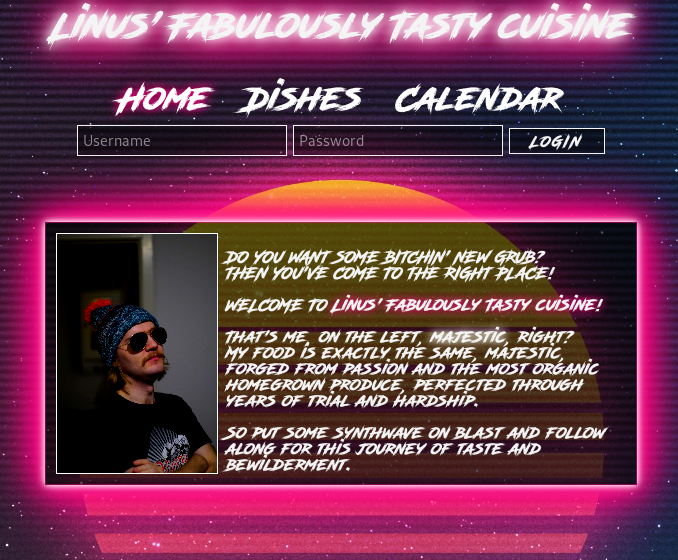
\includegraphics[scale=0.3]{images/login.png}
    \caption{Login, as show on every page.}
    \label{fig:login}
  \end{center}
\end{figure}

\begin{figure}[H]
  \begin{center}
    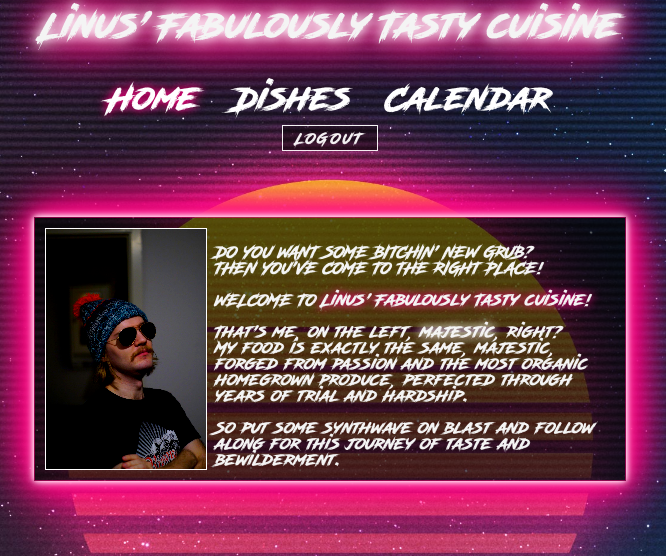
\includegraphics[scale=0.3]{images/logout.png}
    \caption{Logout, as show on every page while logged in.}
    \label{fig:logout}
  \end{center}
\end{figure}

\textbf{\href{https://github.com/linus-dev/KTH-Projects/tree/master/ID1354/2}{Github}}\\\\

\noindent
The solution was a simple login form below the nav bar as
seen in \ref{fig:login} upon logging in, the login form is
switched to the logout as seen in \ref{fig:logout}. Both
of these are displayed on every page to make sure the
user has an easier time logging in or logging out, without
having to redirect themselves to another page.
\\\\
It is important that the login/logout form follows the 5 basic heuristics of
interface design.
\begin{itemize}
\item{Visibility of system status}\\
  The user quite easily can distinguish between begin logged in and logged out,
  there is no dependencies on colours et cetera, so the system status should be
  easily visible to any user.
\item{Match between system and the real world}\\
  There was not a lot text, however the UI speaks for itself, and login/logout
  are quite universal in today's society and easily understood by any user, username and password is also displayed in
  textboxes accordingly.
\item{Consistency and standards}\\
  The login and logout forms are consistent throughout all pages, it remains in
  the same place at all times, and it also conforms to common login form standards,
  such as having a normal username and password form.
\item{Recognition rather than recall}\\
  The users always know if they are logged in or logged out on every page at the same
  location.
\item{Aesthetic and minimalist design}\\
  The login and logout are by all means minimal and fits the aesthetic style of the rest of the website.
\end{itemize}

\begin{figure}[H]
  \begin{center}
    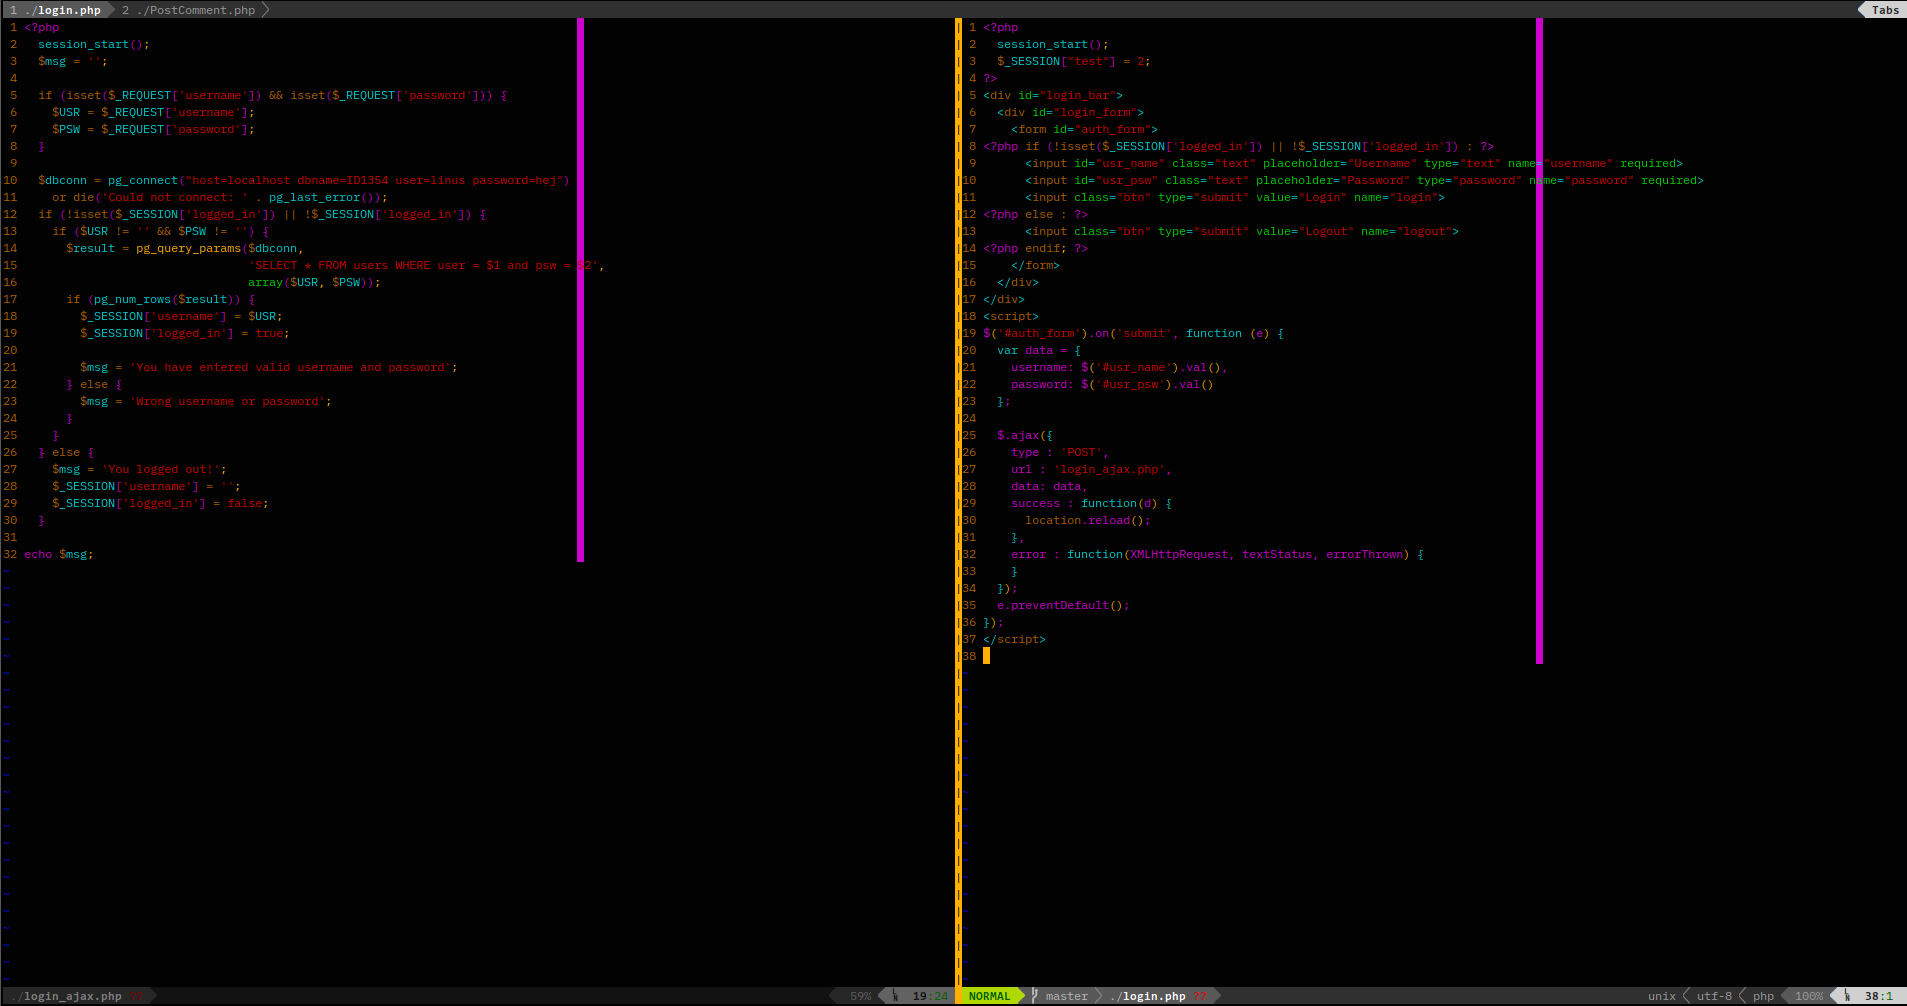
\includegraphics[scale=0.32]{images/login_code.png}
    \caption{login.php and login\_ajax.php}
    \label{fig:login_code}
  \end{center}
\end{figure}

\noindent
For related files see,
\href{https://github.com/linus-dev/KTH-Projects/blob/master/ID1354/2/login_ajax.php}{login\_ajax.php},\\
\href{https://github.com/linus-dev/KTH-Projects/blob/master/ID1354/2/login.php}{login.php}
\\
\\
The login form utilises JQuery, AJAX and PHP to perform both the login and logout,
when the user clicks the login button the JQuery submit hook does an ajax request
to the server for login\_ajax.php with the username and password provided (if this is a logout, they will be null).
\\\\
Upon recieving the request the server checks if the user is logged in or not and basing the next decision
on that (logging in or out). In case the user logs in a database connection is opened and
a simple \textit{SELECT} query is ran to check if there is any such user with that password in the database,
if the database returned anything greater than zero (amount of rows) in the selection, that means a user was found,
the appropriate \textit{SESSION} variables are set and the user is now logged in.
The same as above applies for a logout, except no database connection is made, simply the 
session variables are unset.
The login.php is then included in every page where a login/logout form should be present, like this:

\begin{figure}[H]
  \begin{center}
    
\includegraphics[scale=1]{images/login_include.png}
    \caption{login.php include}
  \end{center}
\end{figure}

\begin{figure}[H]
  \begin{center}
    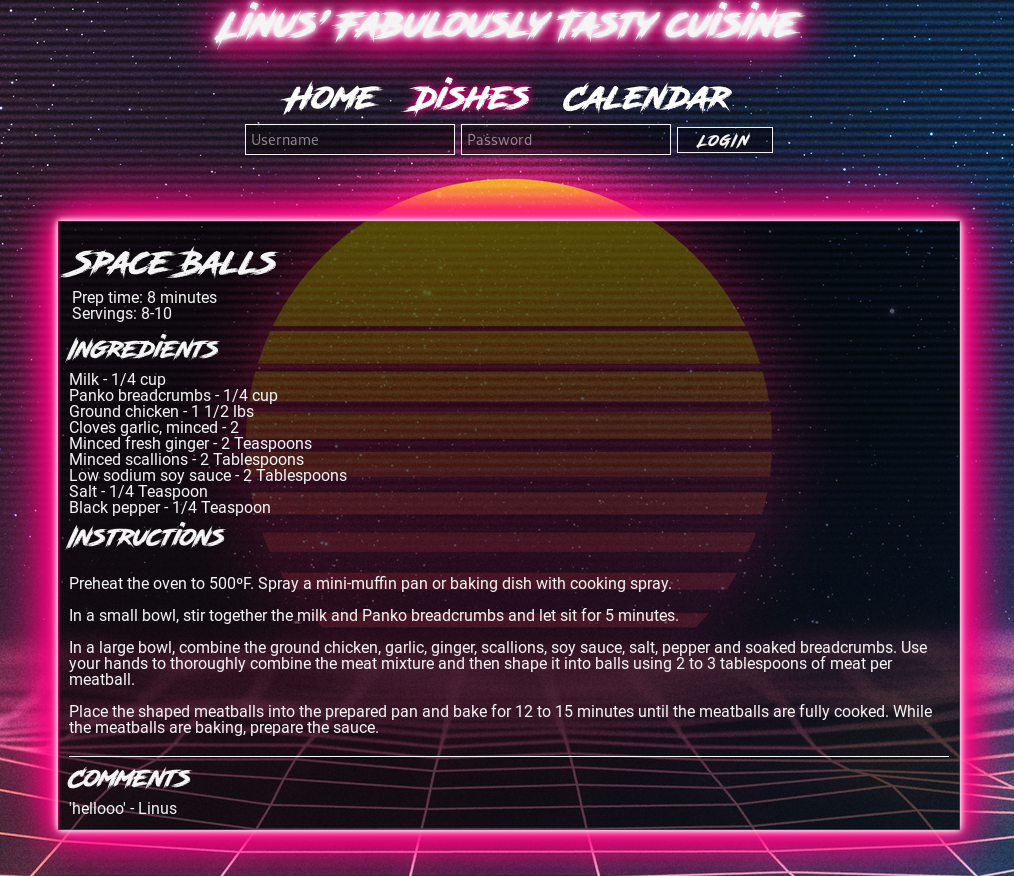
\includegraphics[scale=0.32]{images/comments_logged_out.png}
    \caption{Logged Out}
    \label{fig:cmt_out}
  \end{center}
\end{figure}

\begin{figure}[H]
  \begin{center}
    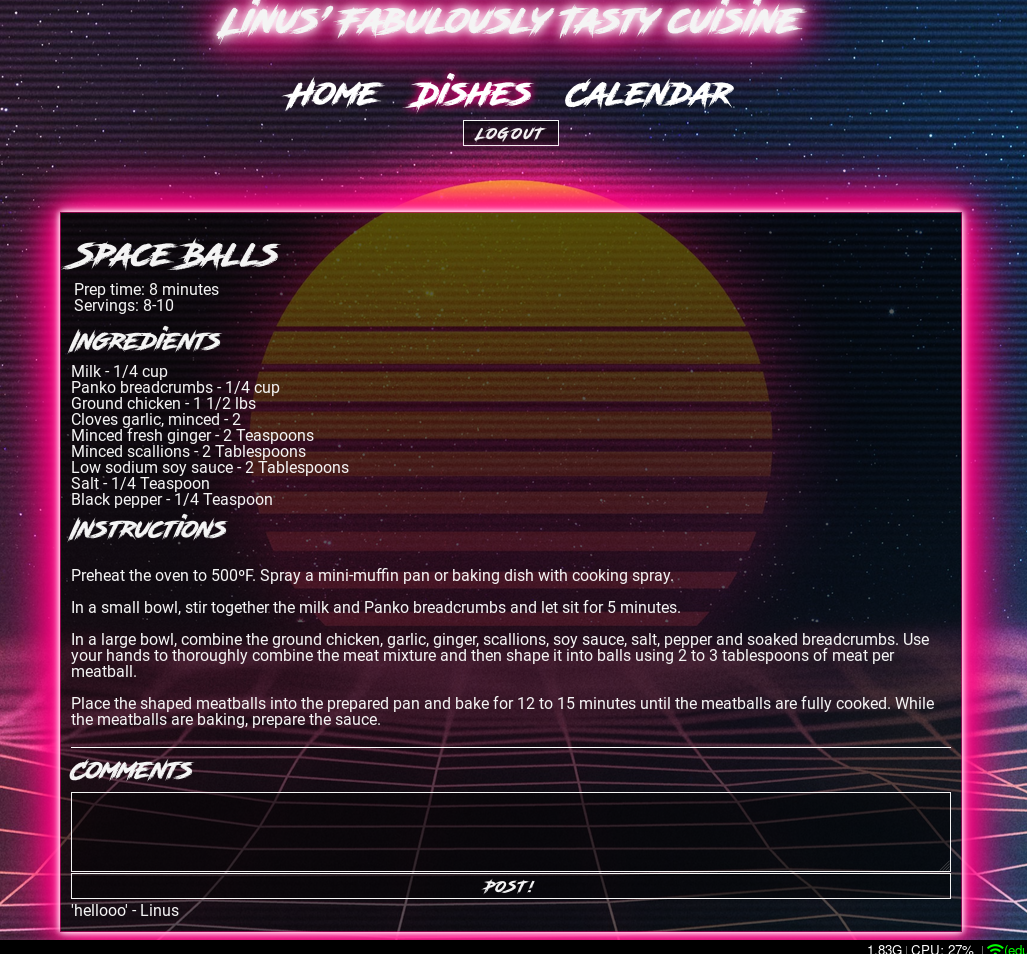
\includegraphics[scale=0.32]{images/comments_logged_in.png}
    \caption{Logged In}
    \label{fig:cmt_in}
  \end{center}
\end{figure}

\begin{figure}[H]
  \begin{center}
    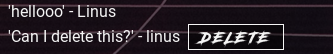
\includegraphics[scale=1]{images/comment_delete.png}
    \caption{Logged In}
    \label{fig:cmt_del}
  \end{center}
\end{figure}

\noindent
As seen in \ref{fig:cmt_out} and \ref{fig:cmt_in} the recipe part of the site displays
different depending on if the user is logged in or not, the comment text box is not
displayed for a guest visitor.
\\\\
In case the user wants to delete a comment posted he or she may easily do so by
clicking the \textit{Delete} button that accompanies each comment as seen in \ref{fig:cmt_del}.
\\\\
\noindent
The comment field is quite simple and intutive.
\begin{itemize}
\item{Visibility of system status}\\
  The user can easily tell if he or she can comment, since it does not display
  if they are not logged in and user will easily be able to tell once he or she
  posts a comment, the page will reload and their comment appears in clear view
  below the comment field.
\item{Match between system and the real world}\\
  'POST!' should be quite a univeral and well understood button, and the text box
  could possibly be a bit more leading/guiding to let the user know where to type,
  however the site feels inutitve enough.
\item{Consistency and standards}\\
  The comment field is the exact same on every recipe, and the user will know
  how to comment if he or she is logged in.
\item{Recognition rather than recall}\\
  The user should quite easily recognize where to comment and what they commented
  due to it instantly displaying.
\item{Aesthetic and minimalist design}\\
  The text field and button are both very simple, it fits the aesthetic of the rest of the site
  and provides enough visual feedback to the user.
\end{itemize}

\begin{figure}[H]
  \begin{center}
    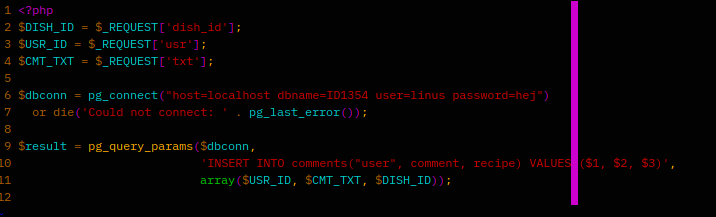
\includegraphics[scale=0.9]{images/cmt_code_post_ajax.png}
    \caption{PostComment.php}
    \label{fig:cmt_post_ajax}
  \end{center}
\end{figure}

\begin{figure}[H]
  \begin{center}
    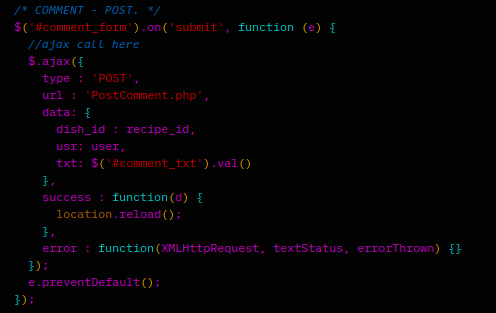
\includegraphics[scale=0.9]{images/cmt_code.png}
    \caption{recipe.php}
    \label{fig:cmt_recipe}
  \end{center}
\end{figure}

\begin{figure}[H]
  \begin{center}
    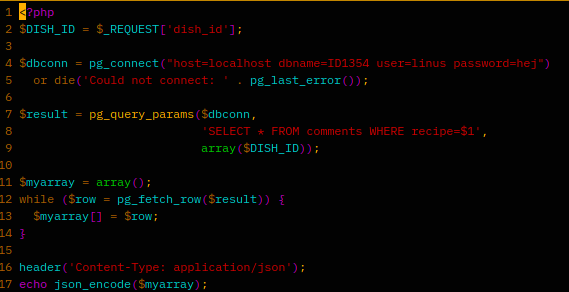
\includegraphics[scale=0.9]{images/cmt_get.png}
    \caption{GetComments.php}
    \label{fig:cmt_get}
  \end{center}
\end{figure}

\begin{figure}[H]
  \begin{center}
    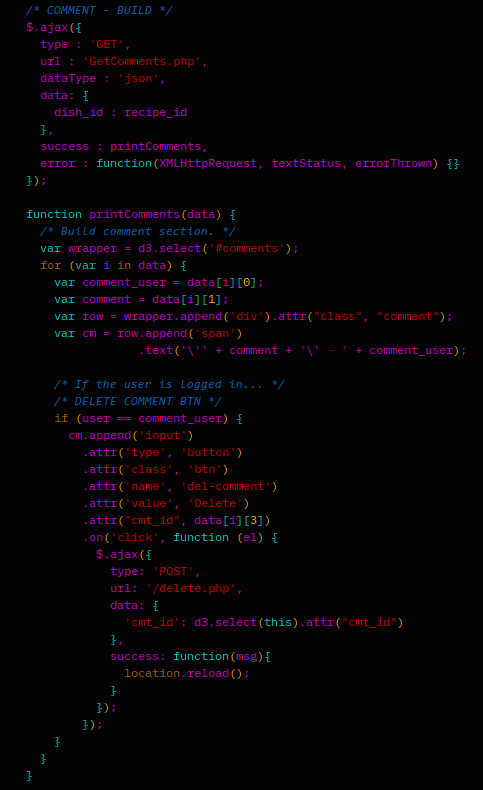
\includegraphics[scale=0.9]{images/cmt_build.png}
    \caption{recipe.php}
    \label{fig:cmt_build}
  \end{center}
\end{figure}

\begin{figure}[H]
  \begin{center}
    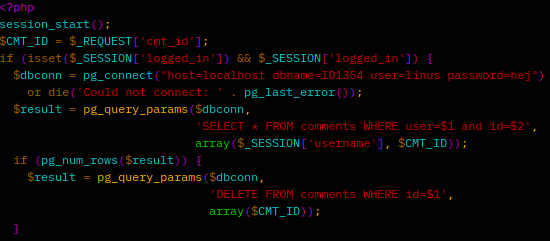
\includegraphics[scale=0.9]{images/cmt_delete.png}
    \caption{delete.php}
    \label{fig:cmt_delete}
  \end{center}
\end{figure}
\noindent
For related files see,\\
\href{https://github.com/linus-dev/KTH-Projects/blob/master/ID1354/2/GetComments.php}{GetComments.php},\\
\href{https://github.com/linus-dev/KTH-Projects/blob/master/ID1354/2/PostComment.php}{PostComment.php},\\
\href{https://github.com/linus-dev/KTH-Projects/blob/master/ID1354/2/delete.php}{delete.php},\\
\href{https://github.com/linus-dev/KTH-Projects/blob/master/ID1354/2/recipe.php}{recipe.php}
\\\\
\noindent
The comment field also utilises JQuery, AJAX, and PHP, in a similar fashion to the login.php file.
\\\\
\noindent
1. Posting a comment.\\
  If the user choses to post a comment, the JQuery submit handle does an ajax request to
  PostComment.php with the recipe ID, user ID, and the text the user posted, as seen in \ref{fig:cmt_recipe}.
  The PostComment.php file does a simple database insert into the PostgreSQL db (\ref{fig:cmt_post_ajax}).
\\\\
2. Getting comments\\
  Getting comments is slightly more interesting because it uses JSON headers and output to
  provide the user with the comments that the server has stored, the client does an AJAX
  request to the server (GetComments.php) with the recipe ID, the server then returns a JSON structure
  with all comments available and builds the comment section with the D3.js library.
\\\\
3. Deleting comments\\
  The user can request a comment to be deleted by pressing the delete button (\ref{fig:cmt_del}),
  this triggers the the D3.js \textit{on click} event which is defined in \ref{fig:cmt_build}.
  The event does an ajax request to delete.php and the server checks to make sure the user is allowed to delete
  said comment and then runs a delete query on the database.
\\\\
Overall the design is very functional, many aspects could be improved and the code right now
is very unstructured, however it works well.
\section{Discussion}

I do not have much to discuss this seminar, other than the obvious security flaws over 
using a well designed system implemented by a dedciated software team, the passwords
are not hashed nor salted, so there is an obvious flaw in storing it as plaintext,
and the website does not utilise a secure connection (SSL). I am also fairly certain
that even though I utilise bindings for the querys, the input should be sanitized more,
there is a large posibility the website is vulnerable to SQL injections, XSS
attacks should not be possible as the comments are escaped, however I only did
basic testing as can be seen in \ref{fig:xss}.
\\
\begin{figure}[H]
  \begin{center}
    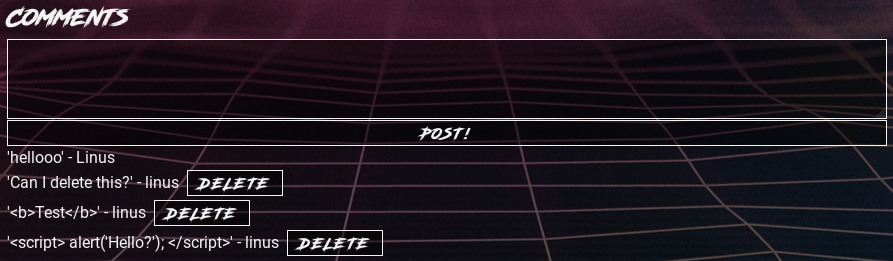
\includegraphics[scale=0.6]{images/xss.png}
    \caption{XSS}
    \label{fig:xss}
  \end{center}
\end{figure}
\noindent
Inadvertedly it appears this solution is the way that seminar four requests us to
implement the user requests, so that turned out great.
\\\\
I could have also solved the optional tasks as they are quite trivial, especially
registration with a database, however procrastination once again was victorious.

\end{document}
